\section{Evaluation}
\label{sec:eval}


\begin{figure}[t]
%\small
\centering
  \begin{tikzpicture}[auto, node distance=.15cm and 0.6cm]

    \node [process, label=left:{Enzyme}] (clang1) {Clang};

    \node [process, right= of clang1] (opt1) {\texttt{-O2}};

    \node [process, right= of opt1] (enzyme1) {Enzyme};

    \node [process, right= of enzyme1] (popt1) {\texttt{-O2}};

    
    \node [process, label=left:{Ref}, below= of clang1] (clang2) {Clang};

    \node [process, below= of enzyme1] (enzyme2) {Enzyme};

    \node [process, right= of enzyme2] (opt2) {\texttt{-O2}};

    \node [process, right= of opt2] (popt2) {\texttt{-O2}};

    \node [process, right= of popt2] (cg2) {CodeGen};

    \node [process, above= of cg2] (cg1) {CodeGen};

    \draw [->, line width=0.5mm] (clang1) -- node {} (opt1);
    \draw [->, line width=0.5mm] (opt1) -- node {} (enzyme1);
    \draw [->, line width=0.5mm] (enzyme1) -- node {} (popt1);
    \draw [->, line width=0.5mm] (popt1) -- node {} (cg1);

    \draw [->, line width=0.5mm] (clang2) -- node {} (enzyme2);
    \draw [->, line width=0.5mm] (enzyme2) -- node {} (opt2);
    \draw [->, line width=0.5mm] (opt2) -- node {} (popt2);
    \draw [->, line width=0.5mm] (popt2) -- node {} (cg2);
  \end{tikzpicture}

\caption{The evaluation pipelines.}
  \label{fig:pipeline}
\end{figure}

We evaluate the Enzyme approach by measuring the runtime of seven benchmarks: the three reverse-mode benchmarks from Microsoft's machine-learning focused ADBench suite, and four additional tests that are technically interesting or represent potential use cases of Enzyme in practice. The ADBench suite includes bundle analysis (BA), a long short term memory model (LSTM), and a gaussian mixture model (GMM). We also differentiate two integrators (Euler, RK4) from the Odeint header-only ODE solver library ~\cite{ahnert2011odeint}; a simple Fast Fourier Fransform (FFT); and finite difference discretized simulation of the 2-dimensional Brusselator system (Bruss) ~\cite{feinberg1987chemical,yu2018mathematical}.

The two integrators are interesting for testing indirect function calls, complicated C++ headers, and foreign ODE solvers. The FFT test is interesting for demonstrating recursive functions. The Brusselator test demonstrates the utility in adjoint sensitivity analysis for ordinary differential equations, a widely applicable method with applications to PDE-constrained optimization~\cite{biegler2003large, li2004adjoint}, control theory~\cite{piasecki1997control}, and scientific machine learning like neural ODE's~\cite{rackauckas2020universal, chen2018neural}


\begin{figure}
    \centering

\begin{tabular}{cc}
\hspace*{-1cm}
\begin{minipage}[T]{0.69\linewidth}
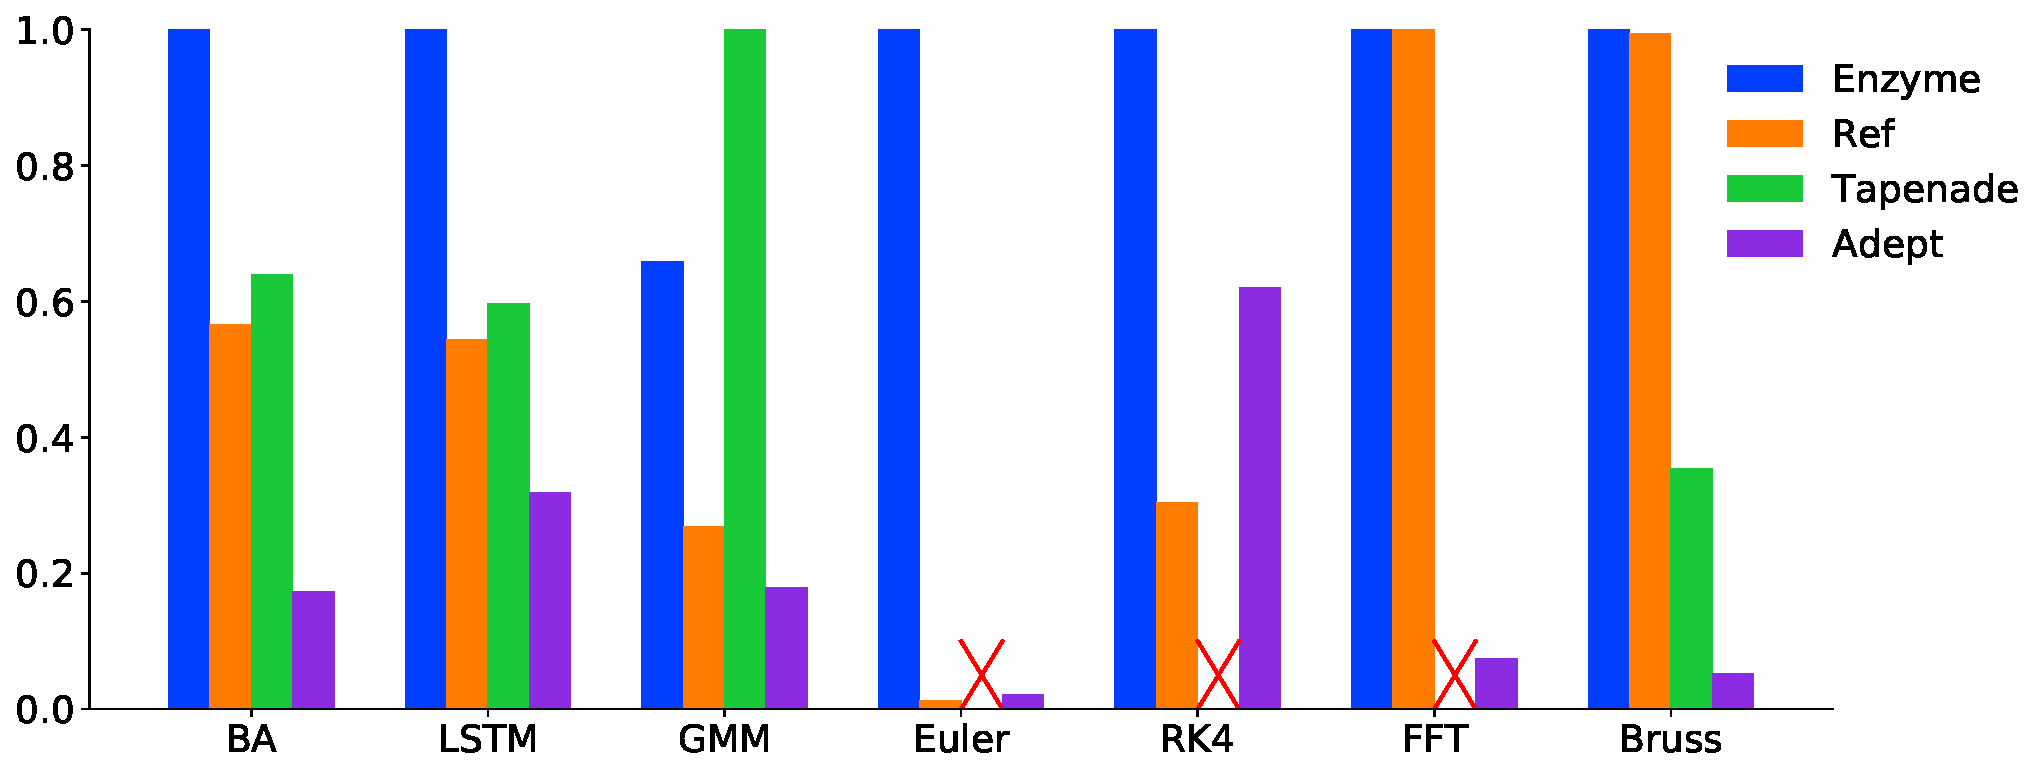
\includegraphics[width=0.99\linewidth]{figs/all.pdf}
\end{minipage}
&
\begin{minipage}[T]{0.29\linewidth}
\hspace*{-1cm} {\scriptsize \begin{tabular}{r|c|c|c|c}
& Enzyme& Ref& Tapenade& Adept\\
BA& \textbf{0.250}& 0.442& 0.391& 1.447\\
LSTM& \textbf{2.405}& 4.426& 4.026& 7.540\\
GMM& 0.261& 0.482& \textbf{0.130}& 0.725\\
Euler& \textbf{0.185}& 14.258& N/A& 8.650\\
RK4& \textbf{3.929}& 12.904& N/A& 6.335\\
FFT& \textbf{0.182}& \textbf{0.182}& N/A& 2.439\\
Bruss& \textbf{0.182}& 0.183& 0.514& 3.444\\
\end{tabular}}
\end{minipage}
\end{tabular}
    \caption{\textbf{\textit{Left:}} Relative speedup of AD systems on the benchmark suite. A red X denotes programs that an AD system does not produce a correct gradient (after accounting for the Tapenade corrections present in ADBench). For each benchmark, we take the geometric mean of the runtime for all test cases, normalizing to the victor. A value of 1.0 denotes the fastest AD system tested for that benchmark, whereas a value of 0.5 denotes that an AD system produced a gradient which took twice as long. \textbf{\textit{Right:}} table with geometric mean runtime in seconds. N/A indicates a benchmark did not work with that system, perhaps producing incorrect results.}
    \label{fig:eval}
\end{figure}

To evaluate the effectiveness of AD on optimized IR, we construct two pipelines shown in Figure~\ref{fig:pipeline}. The Enzyme pipeline consists of running optimizations before Enzyme AD, followed by a second round of optimizations. The Reference (Ref) pipeline is identical to the Enzyme pipeline, except that AD is performed before the first round of optimization. This allows us to effectively evaluate the importance of optimization on AD without considering additional confounding factors (such as differing tape implementations) between Enzyme and existing source AD systems. We ran our experiments on a ``quiesced'' AWS c4.8xlarge instance with hyperthreading and Turbo Boost disabled. Taking the geometric mean across all benchmarks, Enzyme outperforms Reference by a factor of 2.851.

We also compare against the two fastest C/C++ AD tools evaluated in ADBench. These results are presented in Figure~\ref{fig:eval}. Enzyme demonstrate state-of-the-art performance for 7 of the 8 benchmarks. Furthermore the reference pipeline achieves similar performance to Tapenade on the BA and LSTM benchmarks, suggesting that Enzyme's advantage stems from running optimizations first. Tapenade's superior performance on GMM and Enzyme's superior performance on Bruss, however, can be explained by differences in how Enzyme and Tapenade implement their tape structures. Initial optimization also makes a significant impact on the Euler and RK4 tests, explaining much of the performance gap between Enzyme and Adept, whereas Enzyme's efficient tape structure explains its superior performance on FFT.


%We ran our experiments on a ``quiesced'' AWS c4.8xlarge instance with 60 GiB of memory and 18 cores. To minimize variance, we disabled hyperthreading and Turbo Boost.